\section{Harun Ar-Rasyid}
\subsection{Sejarah}
Python diciptakan oleh Guido van Rossum pertama kali di Scitchting Mathematisch Centrum (CWI) di Belanda pada awal tahun 1990-an. Bahasa python terinspirasi dari bahasa pemrograman ABC. Sampai sekarang, Guido masih menjadi penulis utama untuk python, meskipun bersifat open source sehingga ribuan orang juga berkontribusi dalam mengembangkannya.

Pada 1995, Guido pindah ke CNRI di Virginia Amerika sambil terus mengembangkan Python. Versi terakhir yang dirilis adalah 1.6. Pada tahun 2000, pengembang inti Guido dan Python pindah ke BeOpen.com yang merupakan perusahaan komersial dan membentuk BeOpen PythonLabs. Python 2.0 dirilis oleh BeOpen. Setelah menghapus Python 2.0, Guido dan beberapa anggota tim PythonLabs pindah ke DigitalCreations.

Saat ini pengembangan Python terus dilakukan oleh sekelompok programmer yang dikoordinir oleh Guido dan Python Software Foundation. Python Software Foundation adalah organisasi nirlaba yang dibentuk sebagai pemegang hak cipta intelektual Python sejak versi 2.1 dan dengan demikian mencegah Python dimiliki oleh perusahaan komersial. Saat ini distribusi Python telah mencapai versi 2.7.14 dan versi 3.6.3

Nama Python dipilih oleh Guido sebagai nama bahasa ciptaannya karena kecintaan Guido pada acara televisi Flying Circus Monty Python. Oleh karena itu sering ekspresi khas acara sering muncul dalam korespondensi antara pengguna Python.
\subsection{Instalasi Anaconda}
\begin{enumerate}
    \item Pastikan Bahwa Python telah terinstal dilaptop anda.
    \item Jika anda belum punya anaconda, kalian bisa download di https://www.anaconda.com/distribution/#download-section
    \item Kemudian buka installer yang telah di download barusan
    \item Klik next
    \begin{figure}[!htbp]
        \centering
        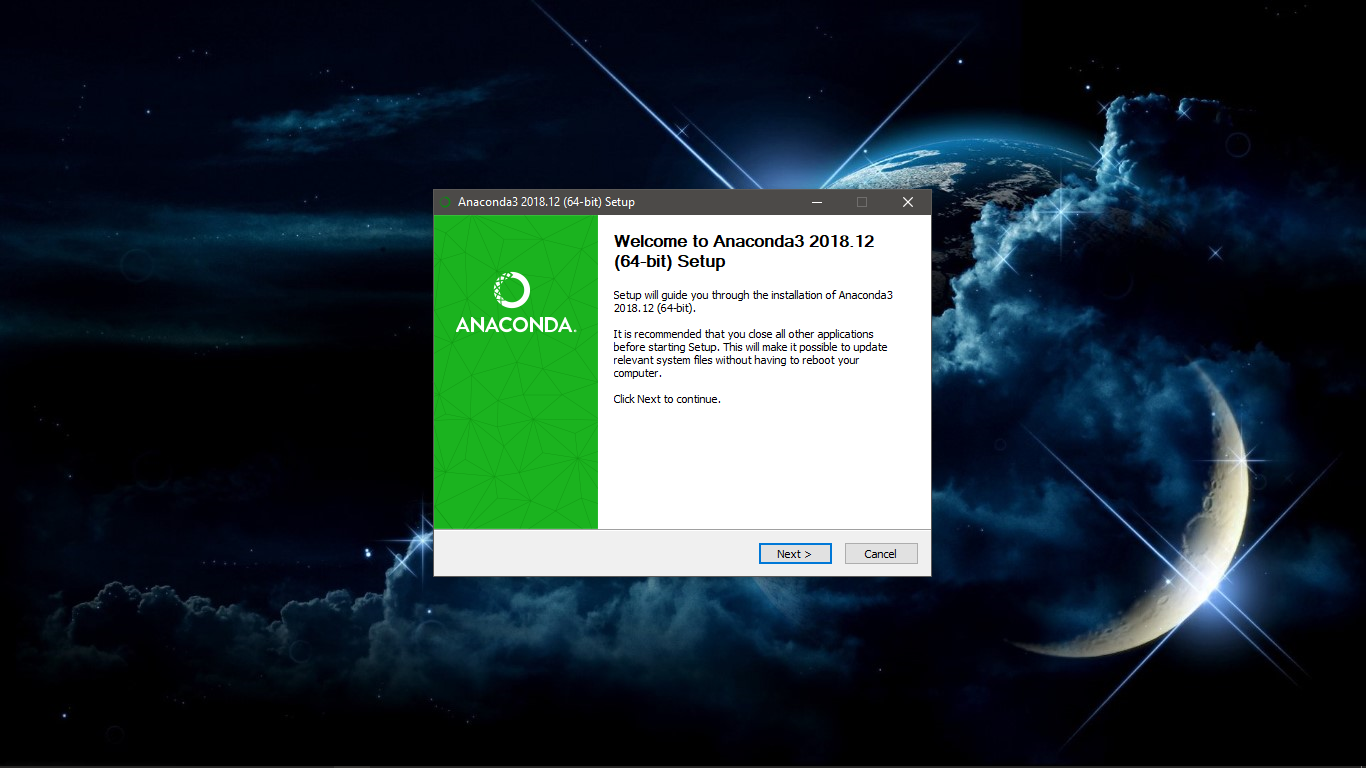
\includegraphics[width=3cm,height=3cm]{figures/Screenshot(80).png}
        \caption{Tampilan Awal}
        \label{awal}
        \end{figure}

    \item Kemudian Klik I Agree
    \begin{figure}[!htbp]
        \centering
        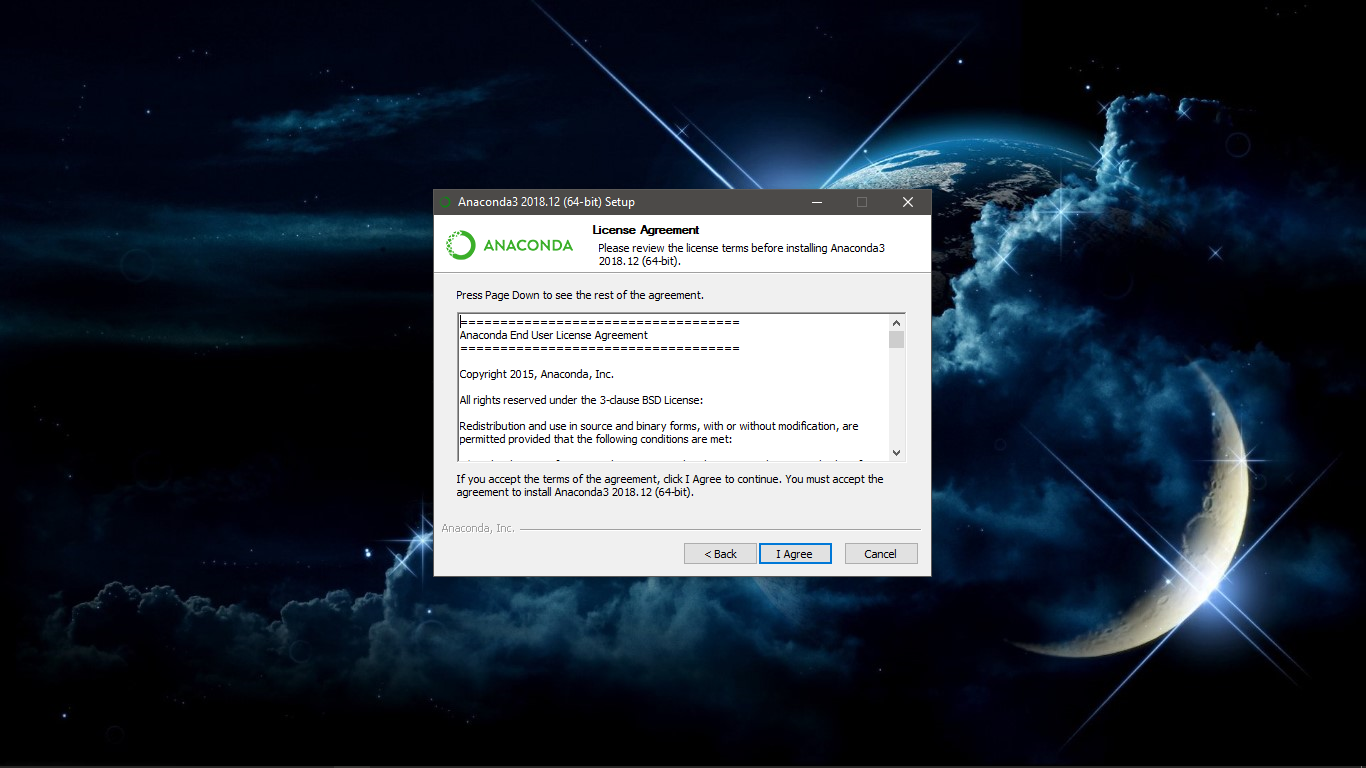
\includegraphics[width=3cm,height=3cm]{figures/Screenshot(81).png}
        \caption{License Agreement}
        \label{License}
        \end{figure}

    \item Kemudian pilih akan di instal untuk siapa, kemudian pilih next
    \begin{figure}[!htbp]
        \centering
        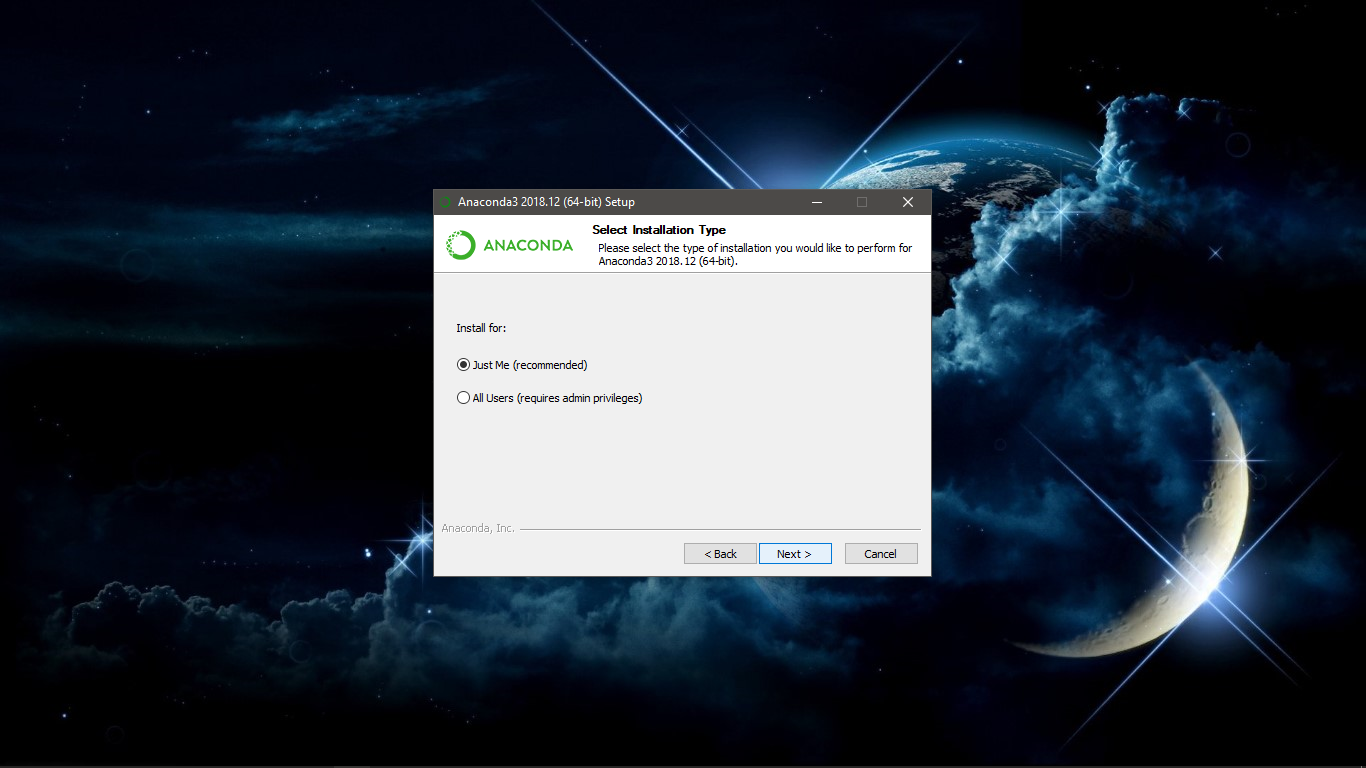
\includegraphics[width=3cm,height=3cm]{figures/Screenshot(82).png}
        \caption{Pemilihan User}
        \label{User}
        \end{figure}

    \item Kemudian tentukan dicretory nya, secara default akan berada di C:\Users\namakomputer\Anaconda3
    \begin{figure}[!htbp]
        \centering
        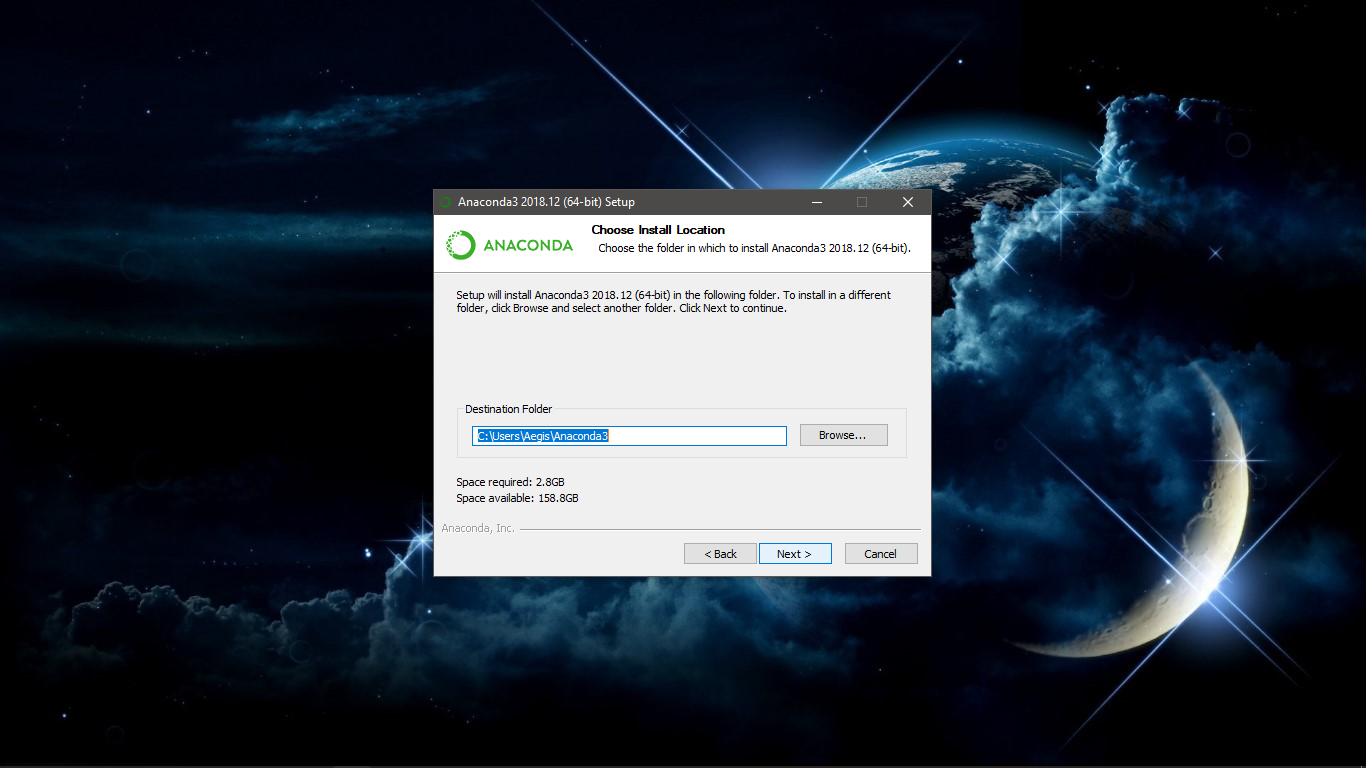
\includegraphics[width=3cm,height=3cm]{figures/Screenshot(83).png}
        \caption{Pemilihan Direktori Penyimpanan}
        \label{Directory}
        \end{figure}

    \item Kemudian Centang yang register Anaconda as default Python, Kemudian Pilih Next
    \begin{figure}[!htbp]
        \centering
        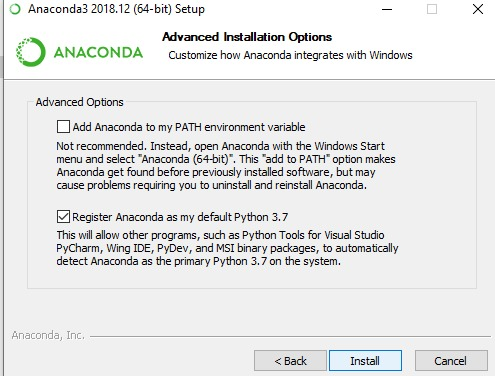
\includegraphics[width=3cm,height=3cm]{figures/Screenshot(84).jpeg}
        \caption{Pemilihan Opsi}
        \label{opsi}
        \end{figure}

    \item Tunggu Proses Instalasi hingga selesai
    \begin{figure}[!htbp]
        \centering
        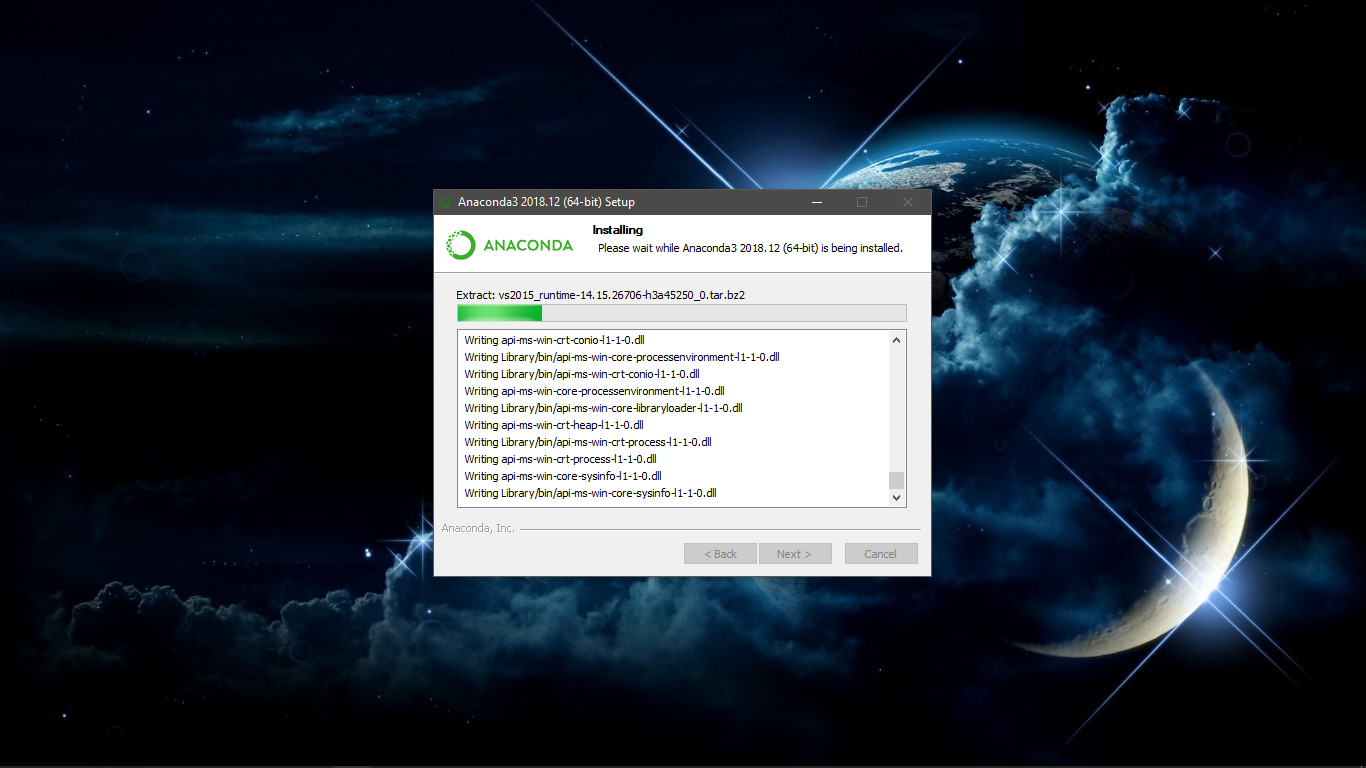
\includegraphics[width=3cm,height=3cm]{figures/Screenshot(85).png}
        \caption{Proses Instal}
        \label{Proses}
        \end{figure}

    \item Klik next
    \begin{figure}[!htbp]
        \centering
        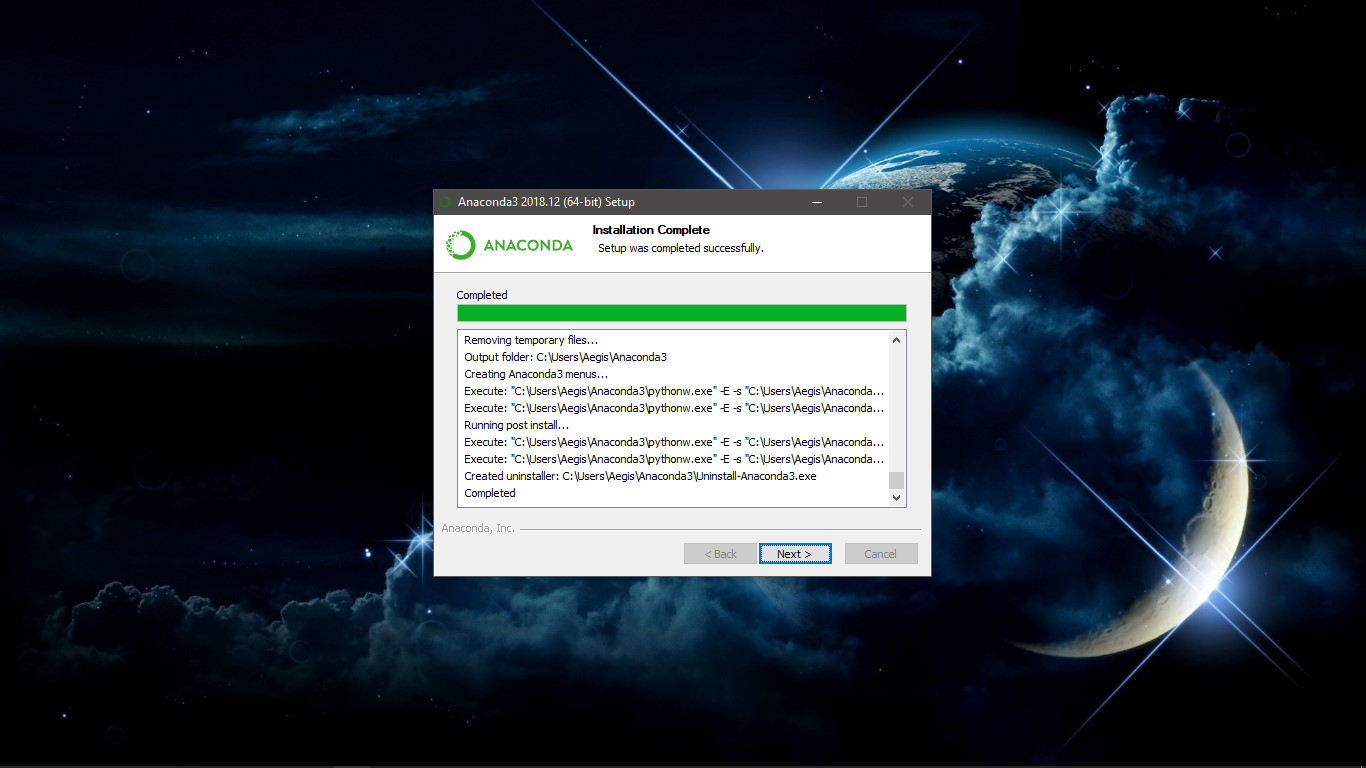
\includegraphics[width=3cm,height=3cm]{figures/Screenshot(86).png}
        \caption{Proses Instal Selesai}
        \label{Proses}
        \end{figure}

    \item kemudian jika kalian belum instal MS VSC di sarankan menginstalnya dlu, jika sudah klik skip
    \begin{figure}[!htbp]
        \centering
        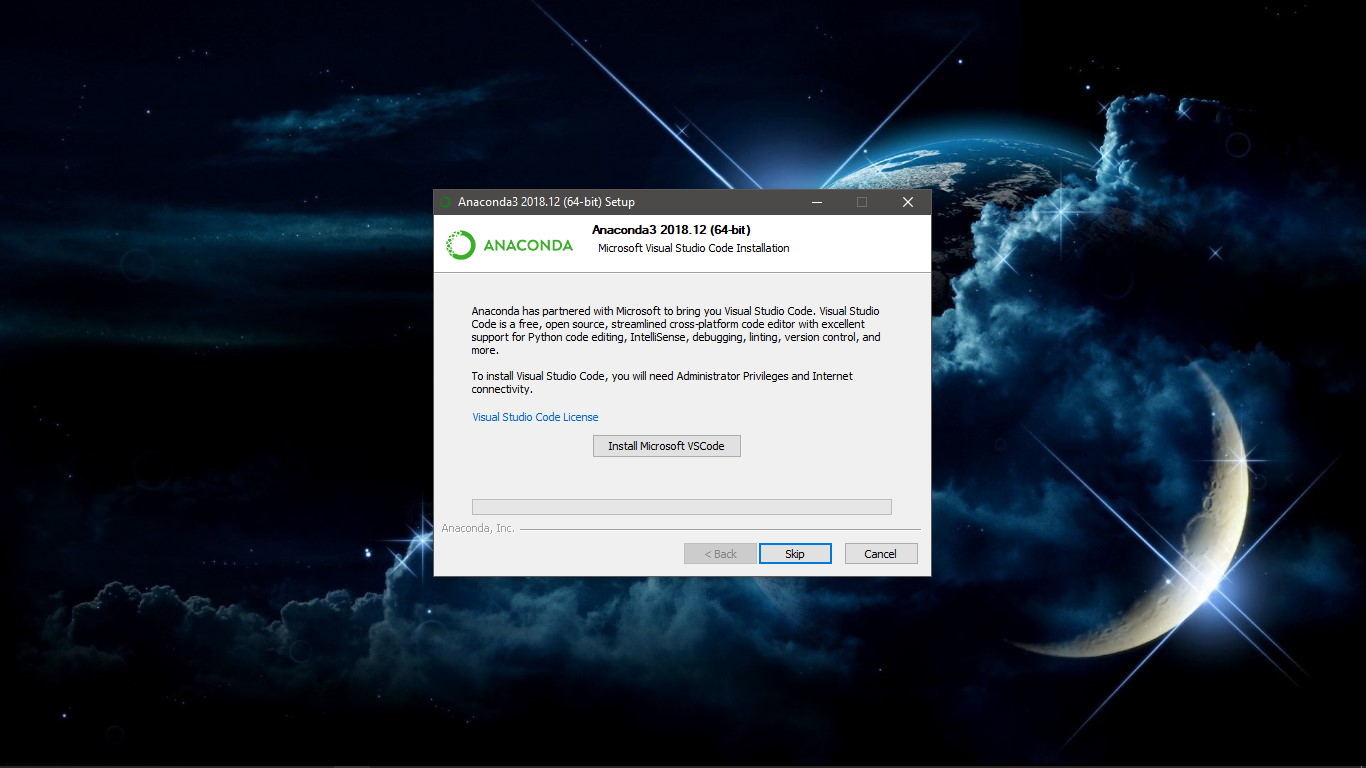
\includegraphics[width=3cm,height=3cm]{figures/Screenshot(87).png}
        \caption{Penawaran Instal MS VSC}
        \label{offering}
        \end{figure}

    \item Instalasi anaconda telah selesai
    \begin{figure}[!htbp]
        \centering
        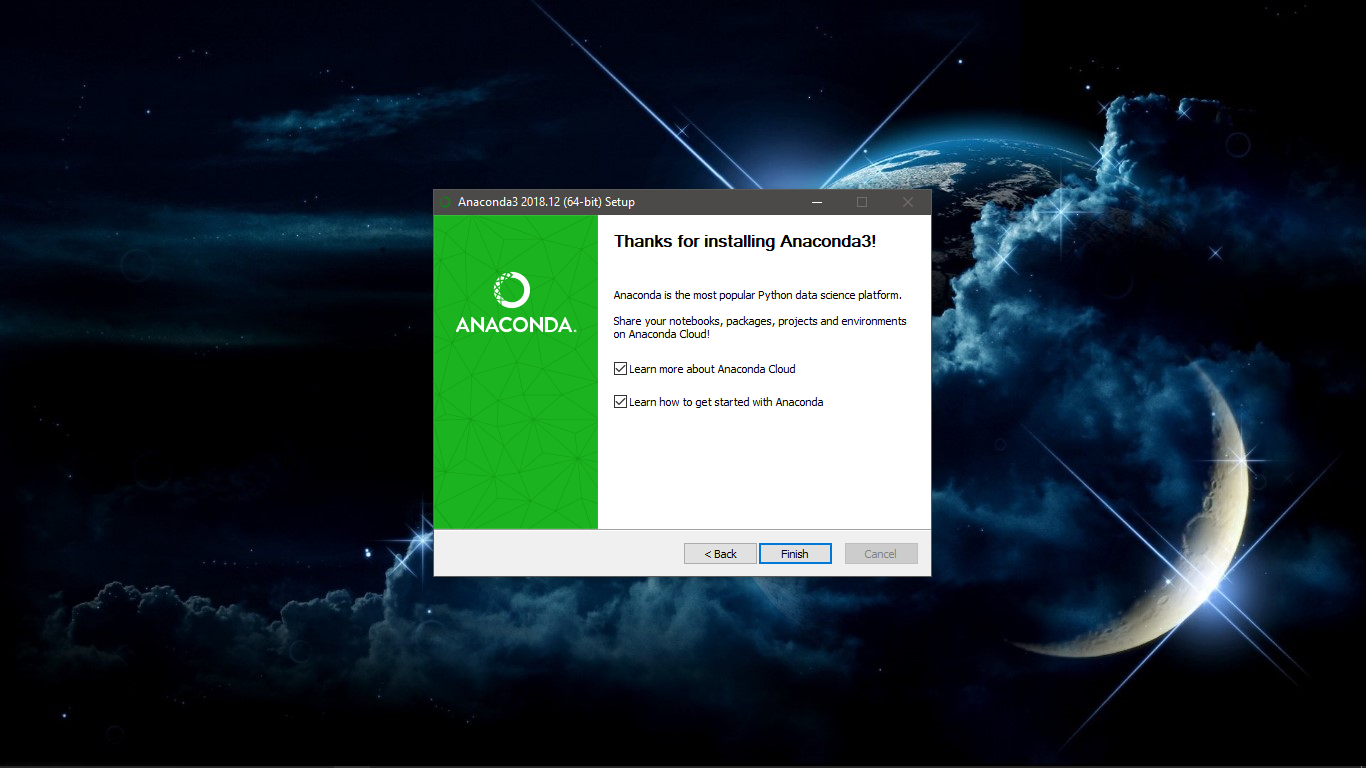
\includegraphics[width=3cm,height=3cm]{figures/Screenshot(88).png}
        \caption{Instalasi Selesai}
        \label{akhir}
        \end{figure}
\end{enumerate}
\subsection{Menggunakan Spyder}
Setelah selesai melakukan instalasi anaconda, maka ada beberapa tool yang digunakan seperti spyder

\begin{figure}[!htbp]
    \centering
    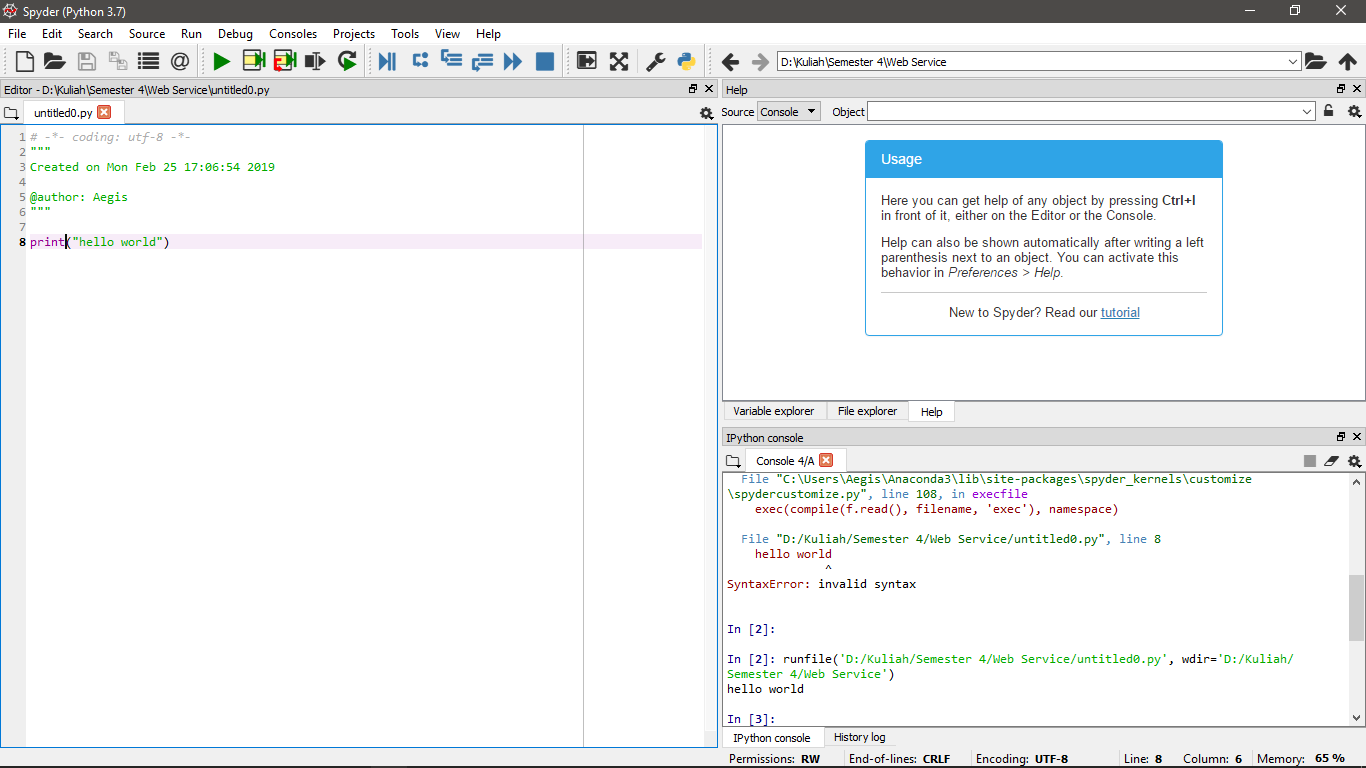
\includegraphics[width=3cm,height=3cm]{figures/Spyder.png}
    \caption{Ini adalah tampilan spyder}
    \label{spyder}
    \end{figure}

Gambar diatas menjelaskan tentang tampilan spider dan mengexsekusi program halo world.